% !TEX program = xelatex
% 基于 CLIP 的图文语义对齐分析报告
\documentclass[12pt,a4paper]{ctexart}

% ---------- 页面设置 ----------
\usepackage[top=2.5cm, bottom=2.5cm, left=2.8cm, right=2.8cm]{geometry}
\usepackage{graphicx}
\usepackage{booktabs}
\usepackage{amsmath}
\usepackage{hyperref}
\usepackage{caption}
\usepackage{float}
\usepackage{enumitem}

\hypersetup{
    colorlinks=true,
    linkcolor=blue,
    urlcolor=blue,
    citecolor=blue
}

\title{\vspace{-1.5em}\Large\bfseries 基于 CLIP 的图文语义对齐分析}
\author{计算机视觉课程大作业 · 实验报告}
\date{\today}

\begin{document}

\maketitle

\begin{abstract}
本实验使用预训练 CLIP（Contrastive Language-Image Pre-training）模型，在不训练、不微调、不使用 CIFAR-10 训练集的前提下，分析图像特征与文本语义在共享 latent space 中的对齐关系。CIFAR-10 zero-shot 分类在本文中被视为一种观测手段：image encoder 将图像映射为视觉特征向量，text encoder 将类别 prompt 映射为文本语义向量，二者通过余弦相似度进行匹配。在 ViT-B/32 baseline 上，Single Generic Prompt 取得 88.33\% 的整体准确率，Generic Multi-template Ensemble 取得 88.99\%；换用 ViT-L/14 后，Single Generic Prompt 达到 95.14\%。在此基础上，本文以 \texttt{cat} 语义为中心，进一步分析 CIFAR-10 图像在 \texttt{cat} 文本锚点附近的聚集情况、细粒度猫类 prompt 的相似度差异、外部猫图像的迁移表现，以及误导性 prompt 对文本锚点的影响。实验结果表明，CLIP 的 zero-shot 能力来自跨模态语义表示的对齐，而不是传统意义上的固定分类头。
\end{abstract}

\newpage
\tableofcontents
\newpage

% ==================== 第一章 ====================
\section{引言}

传统的图像分类任务通常依赖大量人工标注的训练样本，且分类器只能识别训练阶段定义好的固定类别集合。一旦需要增加或更换识别类别，就必须重新收集标注数据并重新训练模型。这种“一类别一训练”的范式在实际应用中成本高昂。

Zero-shot 图像分类的目标是突破这一限制：在不提供目标类别训练样本的情况下，直接对未见过的类别进行分类。实现这一目标的关键在于，模型必须能够理解类别标签的\textbf{语义含义}，而非仅仅记住特定类别的视觉模式。

OpenAI 于 2021 年提出的 CLIP（Contrastive Language-Image Pre-training）模型~\cite{radford2021clip} 为 zero-shot 分类提供了新的范式。CLIP 通过在 4 亿对（图像，文本）数据上进行对比学习，训练出一个 image encoder 和一个 text encoder，将图像和文本映射到同一共享潜在空间。在这一空间中，语义相近的图像和文本会自然靠近，语义无关的则相互远离。于是，分类问题被转化为一个向量检索问题：将待分类图像的特征向量与所有候选类别的文本特征向量逐一比较相似度，选择最匹配的类别即可——整个过程不涉及任何训练或参数更新。

本实验的目标包括：
\begin{enumerate}[label=(\arabic*)]
    \item 理解 CLIP 双塔结构的工作机制：掌握 image encoder、text encoder、shared latent space 和 cosine similarity 在 zero-shot 匹配中的角色；
    \item 用 CIFAR-10 zero-shot 分类观察语义对齐：使用预训练 CLIP 模型对 10,000 张测试图像进行分类，不访问训练集、不进行任何训练或微调；
    \item 围绕 \texttt{cat} 文本锚点分析 latent space 结构：观察 \texttt{cat} 语义附近聚集哪些图像特征，哪些非 cat 对象容易靠近 cat，细粒度 cat prompt 与误导 prompt 如何改变文本锚点位置；
    \item 分析 prompt 对 CLIP 判断的影响：说明 prompt 不是简单标签，而是 text encoder 在共享空间中生成的语义向量；措辞、上下文、否定词和视觉媒介描述都可能改变相似度。
\end{enumerate}

本实验的严格约束条件将在第 4.4 节中详细说明。核心原则是：不使用 CIFAR-10 训练集、不更新 CLIP 模型参数、主实验仅使用所有类别共享的通用 prompt 模板。

% ==================== 第二章 ====================
\section{CLIP 模型原理}

本章介绍 CLIP 的核心机制：对比预训练、双塔架构，以及 zero-shot 分类的推理流程。

\subsection{对比语言-图像预训练}

CLIP 的训练目标不是让模型学会将图像分到某个预定义的类别（如“猫”或“狗”），而是学会判断一段文本描述是否与一张图像的内容相匹配。训练数据为 4 亿对（图像，自然语言描述）样本，涵盖互联网上广泛的主题和场景。

在训练过程中，一个 batch 包含 $N$ 对匹配的（图像，文本）样本。CLIP 学习的目标是：对于每一张图像，让它的特征向量与对应文本描述的特征向量在 latent space 中尽可能靠近，而与 batch 内其他 $N-1$ 条不匹配文本的特征向量尽可能远离。同样地，对于每一条文本，也要与它对应的图像靠近，与不匹配的图像远离。这种“正样本拉近、负样本推远”的训练方式被称为\textbf{对比学习}（contrastive learning）。

与传统的监督图像分类相比，CLIP 的预训练范式有本质区别。监督分类学到的是从图像到固定类别标签的映射；而 CLIP 学到的是图像与文本之间的通用语义对齐关系。正是这一差异，使得 CLIP 具备了在未见类别上进行 zero-shot 迁移的能力。

\subsection{双塔架构}

CLIP 由两个独立的 encoder 组成，称为“双塔”（dual-tower）架构。

\textbf{Image Encoder} 负责将输入图像编码为固定维度的特征向量。CLIP 提供多种 backbone 选择，本实验使用的是基于 Vision Transformer（ViT）~\cite{dosovitskiy2021vit} 的 image encoder。ViT 的处理流程为：将输入图像切分为固定大小的 patch（如 $32\times32$ 或 $14\times14$ 像素），每个 patch 展平后经过线性投影得到 patch embedding，再送入多层 Transformer 自注意力网络，最终输出一个全局图像特征向量。

\textbf{Text Encoder} 负责将文本描述编码为与图像特征同维度的特征向量。CLIP 的 text encoder 基于 Transformer 架构：输入文本首先经过 byte-pair encoding（BPE）tokenization 切分为子词 token，再经过多层自注意力网络，最终输出的文本特征向量与图像特征向量维度相同。这一“维度相同”的设计是 shared latent space 的物理基础。

两个 encoder 在结构上完全独立，唯一的联系在于：它们输出的特征向量被投影到同一个\textbf{共享潜在空间}（shared latent space）中，且两者均经过 L2 归一化，使得向量比较可以在统一的尺度下进行。

值得注意的是，同一 CLIP 模型内 image feature 和 text feature 的维度始终相同，但不同 backbone 的 projection dimension 可以不同。例如，本实验中 ViT-B 系列的 projection dimension 为 512，ViT-L/14 的 projection dimension 为 768。使用不同 backbone 时，需注意 CLIPProcessor 和 feature dimension 均由各模型自身的配置文件决定。

\subsection{Zero-shot 分类推理流程}

在推理阶段，CLIP 的 zero-shot 分类遵循以下四步流程：

\textbf{Step 1 — 构建文本特征}：将 CIFAR-10 的类别名称（如“airplane”、“cat”）嵌入预先设计的 prompt 模板（如 \texttt{"a photo of a \{\}."}），形成完整的自然语言句子。这些文本通过 CLIP text encoder 编码为文本特征向量，再经过 L2 归一化，得到每个类别的 text embedding。若使用多模板集成，对同一类别在不同模板下的 text embedding 取均值后重新 L2 归一化，作为该类的最终 text embedding。

\textbf{Step 2 — 提取图像特征}：将 CIFAR-10 测试图像通过 CLIPProcessor 进行预处理（resize、center crop、to tensor、normalize），送入 CLIP image encoder 编码为图像特征向量，再经过 L2 归一化，得到 image embedding。

\textbf{Step 3 — 计算相似度}：由于 image embedding 和 text embedding 均已 L2 归一化，两者的余弦相似度（cosine similarity）可直接通过向量内积计算：
\begin{equation}
    \text{similarity}(I, T_c) = \hat{\mathbf{v}}_{\text{image}} \cdot \hat{\mathbf{v}}_{\text{text}, c}
\end{equation}
其中 $\hat{\mathbf{v}}_{\text{image}}$ 为归一化后的图像特征向量，$\hat{\mathbf{v}}_{\text{text}, c}$ 为类别 $c$ 的归一化文本特征向量。对于 10 个类别，每张图像得到一个 $(1, 10)$ 的相似度向量。

\textbf{Step 4 — 预测类别}：取相似度最高的类别作为预测结果（argmax）：
\begin{equation}
    \hat{y} = \arg\max_c \; \text{similarity}(I, T_c)
\end{equation}

整个推理过程不涉及反向传播、参数更新或任何形式的训练。Image encoder 和 text encoder 的参数完全冻结（\texttt{model.eval()} + \texttt{torch.no\_grad()}），仅做前向传播。

% ==================== 第三章 ====================
\section{实验方法}

本章详细说明实验的数据集、分类 pipeline、实验设置和评估指标。

\subsection{数据集与预处理}

本实验使用 \textbf{CIFAR-10} 数据集~\cite{krizhevsky2009cifar}。CIFAR-10 包含 60,000 张 $32\times32$ 像素的彩色自然图像，均匀分布在 10 个类别中：airplane、automobile、bird、cat、deer、dog、frog、horse、ship、truck。其中 50,000 张为训练集，10,000 张为测试集，每个类别在测试集中恰好各有 1,000 张。

本实验\textbf{仅使用 CIFAR-10 测试集}（\texttt{train=False}）进行评估，完全不加载或访问训练集数据。

图像预处理遵循 CLIP 的标准流程：输入尺寸调整（resize）、中心裁剪（center crop）、张量转换（to tensor）、归一化（normalize），均由 HuggingFace 的 \texttt{CLIPProcessor} 根据所加载的具体模型配置统一完成。\texttt{CLIPProcessor.from\_pretrained(model\_name)} 会自动读取对应预训练模型的预处理参数（包括目标分辨率、均值、标准差等），确保图像处理与模型训练阶段保持一致。本实验不在 \texttt{data\_loader} 中重复进行 resize、ToTensor 或 normalize，DataLoader 仅返回原始 PIL Image 和对应的类别标签，避免重复预处理带来的特征失真。

\subsection{分类 Pipeline}

分类 pipeline 严格按照第 2.3 节所述的四步流程实现，具体代码实现要点如下：

\textbf{Step 1 — 文本特征构建}：将 10 个 CIFAR-10 类别名称分别嵌入 prompt 模板，生成完整的文本描述。使用 \texttt{CLIPProcessor} 对文本进行 tokenization（padding + truncation），再通过 \texttt{CLIPModel.get\_text\_features()} 编码为文本特征向量。所有 text feature 经过 L2 归一化：$\mathbf{v}_{\text{norm}} = \mathbf{v} / \|\mathbf{v}\|_2$。若使用多模板集成，同一类别在不同模板下的 text feature 先各自 L2 归一化，取算术平均后再次 L2 归一化，得到该类的最终 text embedding，形状为 $(10, \text{feature\_dim})$。

\textbf{Step 2 — 图像特征提取}：对 DataLoader 返回的每一批 PIL Image，使用 \texttt{CLIPProcessor} 统一完成预处理，再通过 \texttt{CLIPModel.get\_image\_features()} 编码为图像特征向量。所有 image feature 同样经过 L2 归一化，形状为 $(\text{batch\_size}, \text{feature\_dim})$。

\textbf{Step 3 — 相似度计算}：归一化后的 image features 与 text features 做矩阵乘法，得到余弦相似度矩阵，形状为 $(\text{batch\_size}, 10)$。

\textbf{Step 4 — 预测}：对每张图像取相似度最高的类别索引：\texttt{predictions = similarity.argmax(dim=-1)}。

关键实现细节：
\begin{itemize}
    \item 整个推理过程包裹在 \texttt{torch.no\_grad()} 上下文管理器中，禁用梯度计算；
    \item 模型设置为 \texttt{model.eval()} 模式，确保 BatchNorm 等层处于推理状态；
    \item 所有 tensor 通过 \texttt{.to(device)} 移动到 GPU（CUDA）或 CPU，视硬件环境而定；
    \item 不使用任何优化器（optimizer）、不调用 \texttt{.backward()}、不保存 checkpoint。
\end{itemize}

\subsection{实验设置}

\textbf{预训练模型}

本实验使用以下 OpenAI CLIP 预训练模型~\cite{huggingface_clip}，均通过 HuggingFace Transformers 库加载：

\begin{table}[H]
\centering
\caption{本实验使用的预训练 CLIP 模型}
\begin{tabular}{lllll}
\toprule
模型标识 & HuggingFace ID & Image Encoder & Patch Size & Projection Dim \\
\midrule
ViT-B/32（baseline）& \texttt{openai/clip-vit-base-patch32} & ViT-B & $32\times32$ & 512 \\
ViT-B/16            & \texttt{openai/clip-vit-base-patch16} & ViT-B & $16\times16$ & 512 \\
ViT-L/14            & \texttt{openai/clip-vit-large-patch14} & ViT-L & $14\times14$ & 768 \\
\bottomrule
\end{tabular}
\end{table}

所有模型在加载时即设置为 eval 模式，不进行任何 fine-tune。

\textbf{主实验 Prompt 策略（严格 zero-shot）}

主实验仅使用所有 10 个类别\textbf{共享}的通用 prompt 模板。共两组策略：

\begin{itemize}
    \item \textbf{Single Generic Prompt}：仅使用 1 条模板 \texttt{"a photo of a \{\}."}
    \item \textbf{Generic Multi-template Ensemble}：使用 8 条通用模板，对同一类别在不同模板下的 text feature 取平均：
    \begin{quote}
    \texttt{"a photo of a \{\}."}\\
    \texttt{"a blurry photo of a \{\}."}\\
    \texttt{"a low resolution photo of a \{\}."}\\
    \texttt{"a photo of a small \{\}."}\\
    \texttt{"a photo of a large \{\}."}\\
    \texttt{"a close-up photo of a \{\}."}\\
    \texttt{"a bright photo of a \{\}."}\\
    \texttt{"a dark photo of a \{\}."}
    \end{quote}
\end{itemize}

\textbf{扩展实验}：模型规模对比（使用 Single Generic Prompt，ViT-B/32 vs ViT-B/16 vs ViT-L/14），旨在观察模型容量和 patch size 对 zero-shot 性能的影响。

\textbf{推理环境}
\begin{itemize}
    \item Python 3.11 + PyTorch 2.6.0（CUDA 12.4）
    \item GPU：NVIDIA GeForce RTX 3070 Laptop GPU（8 GB VRAM），无 GPU 时回退 CPU
    \item 批量大小：ViT-B 系列 batch\_size=64，ViT-L/14 batch\_size=32
    \item 所有实验使用 \texttt{torch.no\_grad()} 进行纯前向推理
\end{itemize}

\subsection{评估指标}

本实验使用以下评估指标（通过 scikit-learn 计算）：

\begin{itemize}
    \item \textbf{Overall Accuracy}：$\text{Accuracy} = \frac{\text{正确预测数}}{10,000}$
    \item \textbf{Per-class Accuracy}：每个类别 1,000 张图像各自的分类正确率
    \item \textbf{混淆矩阵}（Confusion Matrix）：$10\times10$ 矩阵，$(i, j)$ 位置表示真实类别为 $i$ 而被预测为类别 $j$ 的样本数
    \item \textbf{分类报告}：包含每个类别的 Precision、Recall 和 F1-score：
    \begin{equation}
        \text{Precision} = \frac{TP}{TP + FP}, \quad
        \text{Recall} = \frac{TP}{TP + FN}, \quad
        F1 = 2 \times \frac{\text{Precision} \times \text{Recall}}{\text{Precision} + \text{Recall}}
    \end{equation}
\end{itemize}

\subsection{以 Cat 为中心的语义邻域分析}

为了从“分类是否正确”进一步转向“语义空间如何组织”，本文选取 CIFAR-10 中的 \texttt{cat} 作为重点分析对象。与传统分类器不同，CLIP 在推理阶段并没有专门针对 \texttt{cat} 的分类头；文本 \texttt{"a photo of a cat."} 经 text encoder 编码后，是共享表示空间中的一个语义锚点。若 CLIP 的跨模态表示确实完成了语义对齐，则真实猫图像应整体靠近该文本锚点；同时，与猫在外观或语义上相近的对象（如 dog）也可能比 airplane、ship 等远距离类别更容易进入该邻域。

围绕这一问题，本文设计了四组补充分析：

\begin{itemize}
    \item \textbf{Cat 语义邻域}：对 CIFAR-10 测试集全部 10,000 张图像提取 image embedding，计算每张图像与 \texttt{cat} 文本锚点的 cosine similarity，并按相似度排序。
    \item \textbf{Cat / dog / deer / horse 可视化}：选取与 cat 容易混淆或同属动物语义域的类别，将图像 embedding 与文本 embedding 共同投影到二维 PCA 空间，观察文本锚点和图像簇的相对位置。
    \item \textbf{细粒度 cat prompt}：比较 \texttt{domestic cat}、\texttt{tabby cat}、\texttt{Persian cat}、\texttt{Siamese cat}、\texttt{kitten}、\texttt{wild cat} 等 prompt 在 CIFAR-10 cat 图像上的相似度分布。
    \item \textbf{外部猫图与误导 prompt}：使用普通外部猫图和 ImageNet 类别风格的猫图检验迁移表现，并比较 \texttt{dog-like cat}、\texttt{toy cat}、\texttt{cartoon cat}、\texttt{not a cat} 等 prompt 与普通 cat prompt 的相似度差异。
\end{itemize}

上述分析均保持与主实验相同的 zero-shot 约束：CLIP 参数冻结，只进行前向推理；CIFAR-10 训练集不被加载；外部图像仅作为评估样本，不用于 prompt 调优或模型选择。

% ==================== 第四章 ====================
\section{实验结果与分析}

本章所有准确率、recall、F1-score、混淆矩阵和 cat-centered 分析数据均来自真实实验输出；没有实验记录支撑的数值不纳入结论。

\subsection{主实验：Zero-shot 分类结果（ViT-B/32 Baseline）}

表~\ref{tab:vitb32-overall} 展示了 ViT-B/32 在两种通用 prompt 策略下的整体分类准确率。

\begin{table}[H]
\centering
\caption{ViT-B/32 Zero-shot 分类 Overall Accuracy}
\label{tab:vitb32-overall}
\begin{tabular}{lc}
\toprule
Prompt 策略 & Overall Accuracy \\
\midrule
Single Generic Prompt（\texttt{"a photo of a \{\}."}）& 88.33\% \\
Generic Multi-template Ensemble（8 templates）& 88.99\% \\
\bottomrule
\end{tabular}
\end{table}

Multi-template Ensemble 相比 Single Prompt 提升了 0.66 个百分点。这说明用多个语义相近但表述不同的模板对 text feature 取平均，可以小幅增强类别 embedding 的鲁棒性，部分抵消单一模板措辞偏差带来的影响。提升幅度有限但方向一致——对于 ViT-B/32 这个规模较小的 backbone 而言，prompt ensemble 是一项低成本的稳定性改进。

CIFAR-10 的随机猜测准确率为 10\%（10 类均匀分布）。ViT-B/32 在完全不使用训练样本的情况下取得了 88.99\% 的准确率，远超随机基线，验证了 CLIP 在 zero-shot 迁移上的有效性。

\begin{table}[H]
\centering
\caption{ViT-B/32 Multi-template Ensemble 分类报告}
\label{tab:vitb32-report}
\begin{tabular}{lrrrrr}
\toprule
类别 & Precision & Recall & F1-score & Support \\
\midrule
airplane   & 0.9583 & 0.8960 & 0.9261 & 1000 \\
automobile & 0.9264 & 0.9440 & 0.9351 & 1000 \\
bird       & 0.8271 & 0.8850 & 0.8551 & 1000 \\
cat        & 0.8276 & 0.8590 & 0.8430 & 1000 \\
deer       & 0.9088 & 0.7970 & 0.8492 & 1000 \\
dog        & 0.8241 & 0.8900 & 0.8558 & 1000 \\
frog       & 0.9791 & 0.7500 & 0.8494 & 1000 \\
horse      & 0.8392 & 0.9710 & 0.9003 & 1000 \\
ship       & 0.9157 & 0.9670 & 0.9407 & 1000 \\
truck      & 0.9381 & 0.9400 & 0.9391 & 1000 \\
\midrule
\textbf{Overall} & --- & --- & \textbf{0.8899} & \textbf{10000} \\
\bottomrule
\end{tabular}
\end{table}

从表~\ref{tab:vitb32-report} 可以看出各类别的表现差异：

\begin{itemize}
    \item \textbf{表现最优的类别}：horse（recall 97.1\%）、ship（recall 96.7\%）、automobile（recall 94.4\%）。这三类的共同特点是具有鲜明且稳定的整体轮廓特征，即使在 $32\times32$ 的低分辨率下也不易与其它类别混淆。
    \item \textbf{表现最差的类别}：frog（recall 75.0\%）、deer（recall 79.7\%）。CIFAR-10 的 $32\times32$ 极低分辨率使 frog 的判别性视觉特征（如皮肤纹理、眼睛细节）难以被有效提取，加上 frog 图像的背景复杂度、姿态变化和颜色变化都比较大，进一步增加了识别难度。deer 主要与 horse 混淆，两者在低分辨率下的四足动物轮廓相似，CLIP 缺乏足够细粒度的纹理信息来可靠地区分它们。
    \item \textbf{Precision 与 Recall 的 trade-off}：frog 的 precision 高达 0.979 但 recall 仅 0.750——这意味着 CLIP 对 frog 的 text embedding 非常“精确”（几乎不会将其它类别误判为 frog），但对 frog 图像的 image embedding 不够好（大量真正的 frog 图像被分到了 bird、dog 等类别）。这说明在该任务中，frog 的文本描述是准确的，但低分辨率图像的视觉信号不足以有效地映射到文本描述所在的 latent space 位置。
\end{itemize}

\textbf{混淆矩阵分析}：混淆矩阵图像已由实验代码保存至输出目录。主要混淆模式包括：frog $\to$ bird（frog 最常见的误分类方向）、deer $\leftrightarrow$ horse（双向混淆）、cat $\leftrightarrow$ dog（双向混淆）、bird $\to$ dog。这些混淆模式基本符合直觉——它们在视觉语义空间中本身就是相近的概念。

\subsection{扩展实验：模型规模对比}

为了探究模型容量和 patch size 对 zero-shot 分类性能的影响，本实验在 Single Generic Prompt 条件下对比了三个 CLIP 预训练模型的分类准确率。

\begin{table}[H]
\centering
\caption{不同 CLIP 模型的 Zero-shot 分类准确率（Single Generic Prompt）}
\label{tab:model-comparison}
\begin{tabular}{llll}
\toprule
模型 & Patch Size & Feature Dim & Overall Accuracy \\
\midrule
ViT-B/32（baseline）& $32\times32$ & 512 & 88.33\% \\
ViT-B/16            & $16\times16$ & 512 & 90.12\% \\
ViT-L/14            & $14\times14$ & 768 & 95.14\% \\
\bottomrule
\end{tabular}
\end{table}

三个模型在准确率上呈明显的阶梯式上升趋势，ViT-L/14 相比 ViT-B/32 baseline 提升了 6.81 个百分点。

分析提升的来源：

\begin{enumerate}
    \item \textbf{Patch Size 的影响}：ViT-B/32 的 patch size 为 $32\times32$，对于 CLIP 标准输入分辨率 $224\times224$，仅切出 $7\times7=49$ 个 patch。这意味着 CIFAR-10 原图（$32\times32$）被放大 7 倍后，每个 $32\times32$ 的 patch 包含的图像细节极为有限。ViT-B/16（patch=16）产生 $14\times14=196$ 个 patch，ViT-L/14（patch=14）产生 $16\times16=256$ 个 patch，patch 粒度更细使得模型能捕获更多局部纹理和形状信息。
    \item \textbf{模型容量的影响}：ViT-L 对比 ViT-B 有更深的 transformer 层数和更宽的特征维度（768 vs 512），更大的模型 capacity 提供了更强的语义表征能力，使文本和图像在 latent space 中的对齐更加精确。
    \item \textbf{对弱势类别的改善}：frog 的 recall 从 ViT-B/32 的 75.0\% 提升至 ViT-L/14 的 85.7\%（提升 10.7 个百分点），deer 从 79.7\% 提升至 94.8\%（提升 15.1 个百分点）。这印证了更大模型和更细 patch 粒度在低分辨率场景下的关键作用——当输入信号本身的判别信息不足时，更强的 encoder 能更有效地从有限像素中抽取结构化的视觉特征。
\end{enumerate}

需要指出的是，ViT-L/14 的推理速度明显慢于 ViT-B/32（约 1.1 it/s vs 约 7.5 it/s），在实际部署中需权衡精度与效率。

\subsection{错误分析}

本节分析基于 ViT-B/32 Multi-template Ensemble 实验的 1,101 个错误分类样本。主要混淆模式及可能的解释：

\begin{itemize}
    \item \textbf{frog $\to$ bird（最常见）}：在 $32\times32$ 低分辨率下，小型动物的轮廓和颜色分布容易共享相似的低频特征。青蛙和鸟类在 CIFAR-10 中可能都有绿色或棕色的背景环境，加剧了混淆。
    \item \textbf{deer $\leftrightarrow$ horse}：两类同为四足哺乳动物，身体比例和站姿在低分辨率下高度相似。ViT-B/32 的 coarse patch 粒度使得模型难以提取毛色、角形等细节差异。
    \item \textbf{cat $\leftrightarrow$ dog}：经典视觉分类难题，两者外观特征本就有大量重叠。即使在 ImageNet 训练的监督模型上，猫狗混淆也是常见现象。
\end{itemize}

从错误分析中也可以反推 CLIP 的分类机制：它做判断时依赖的是图像整体与文本描述之间的全局语义匹配，而非特定的局部特征（如“猫有竖瞳”、“青蛙有蹼”）。当低分辨率抹去了这些局部细节，CLIP 只能依据整体轮廓和颜色分布做判断，而这恰好是容易发生类别间混淆的维度。

\subsection{Cat 语义邻域与图文对齐分析}

本节将分类结果进一步转化为 latent space 分析。核心问题不再是“是否能分到某个类别”，而是：当文本端给出 \texttt{"a photo of a cat."} 时，哪些图像特征会在共享空间中靠近这一文本语义锚点。

首先，从主实验结果可以得到一个总体信号：CIFAR-10 cat 类在 ViT-B/32 Multi-template Ensemble 下 recall 为 85.9\%，precision 为 82.76\%；主要混淆方向包含 cat $\leftrightarrow$ dog。这说明 \texttt{cat} 文本锚点能够吸引大部分真实 cat 图像，但它周围并非只存在 cat 图像，还会出现与 cat 在外观、语义或图文共现上接近的对象。

表~\ref{tab:cat-neighborhood} 展示了不同真实类别图像与 \texttt{cat} 文本锚点的平均相似度。可以看到，真实 cat 图像的平均相似度最高（0.2583）；在非 cat 类别中，dog 的平均相似度最高（0.2272），高于 airplane、ship、truck 等语义距离较远的类别。这说明 CLIP 的 latent space 具有连续语义结构：相似对象在空间中更容易靠近，而不是被硬性分割成互不相关的离散标签。

\begin{table}[H]
\centering
\caption{不同真实类别到 \texttt{cat} 文本锚点的相似度}
\label{tab:cat-neighborhood}
\begin{tabular}{lrr}
\toprule
真实类别 & 平均 cat 相似度 & 前 100 个非 cat 近邻数量 \\
\midrule
cat        & 0.2583 & --- \\
dog        & 0.2272 & 47 \\
frog       & 0.2235 & 24 \\
deer       & 0.2164 & 13 \\
bird       & 0.2163 & 14 \\
horse      & 0.2048 & 2 \\
airplane   & 0.1930 & 0 \\
automobile & 0.1881 & 0 \\
ship       & 0.1863 & 0 \\
truck      & 0.1854 & 0 \\
\bottomrule
\end{tabular}
\end{table}

从排序结果看，cat 相似度最高的前 100 张 CIFAR-10 测试图像中有 91 张真实标签为 cat；前 500 张中有 445 张为 cat。对最接近 cat 锚点的前 100 个非 cat 样本进一步统计，dog 占 47 个，frog 占 24 个，deer 占 13 个，bird 占 14 个，horse 占 2 个，而 airplane、automobile、ship、truck 均为 0。该结果与混淆矩阵中的 cat $\leftrightarrow$ dog 现象互相印证：CLIP 在做判断时依赖的是全局语义匹配，低分辨率图像中的局部纹理不足时，语义相近的动物类更容易靠近同一文本锚点。

\begin{figure}[H]
\centering
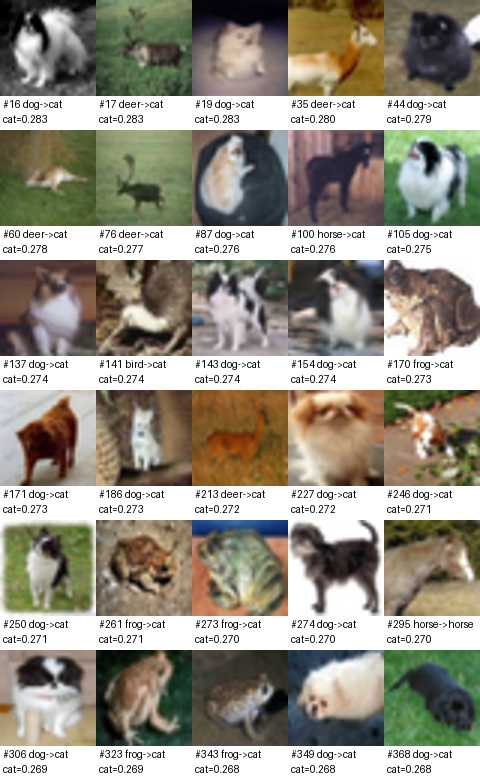
\includegraphics[width=0.88\textwidth]{../outputs/cat_alignment/cat_nearest_non_cat_montage.png}
\caption{最接近 \texttt{cat} 文本锚点的非 cat 图像示例}
\label{fig:cat-nearest-noncat}
\end{figure}

\begin{figure}[H]
\centering
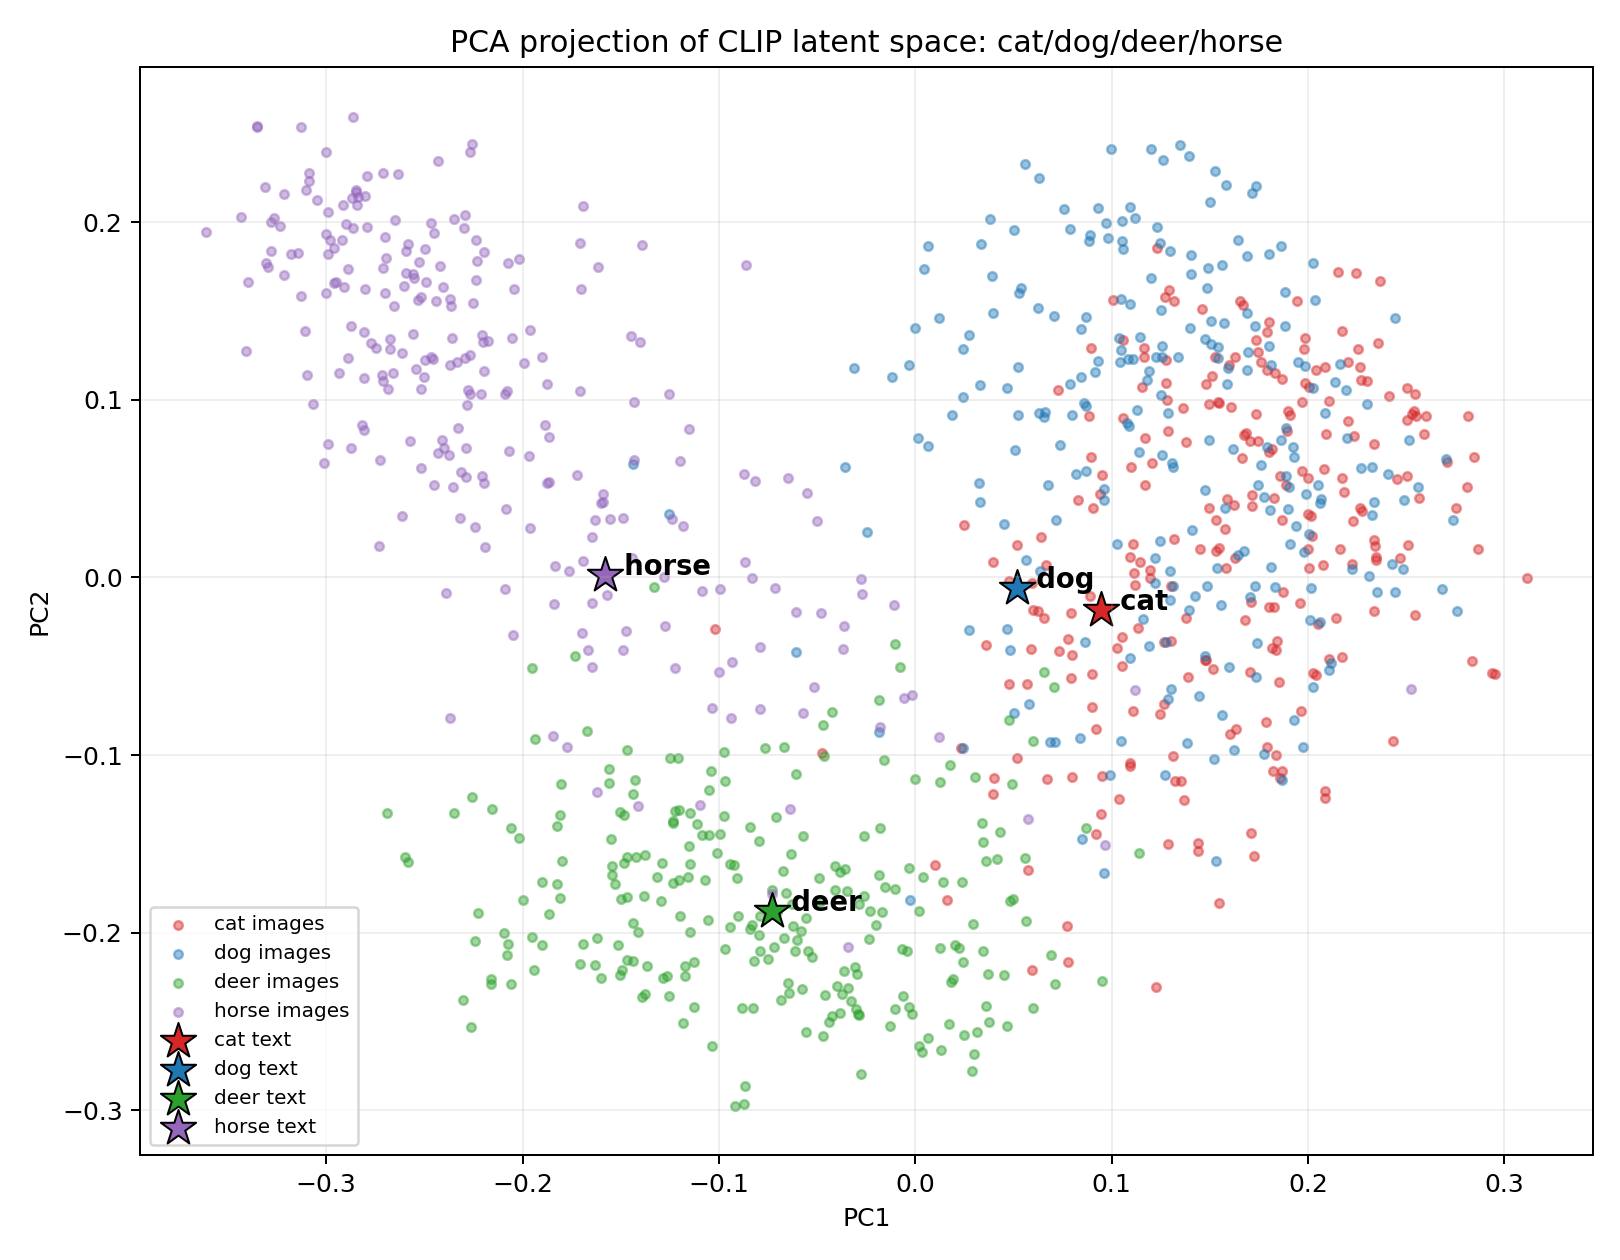
\includegraphics[width=0.82\textwidth]{../outputs/cat_alignment/cat_dog_deer_horse_pca.png}
\caption{cat、dog、deer、horse 图像特征与文本锚点的 PCA 可视化}
\label{fig:cat-pca}
\end{figure}

细粒度 cat prompt 的结果进一步说明，文本 prompt 并不是简单的类别名称，而是在 shared latent space 中产生具体语义位置。表~\ref{tab:fine-cat-prompts} 显示，在 CIFAR-10 的 1000 张 cat 图像上，\texttt{domestic cat} 的平均相似度最高，且在 86.6\% 的 cat 图像中成为细粒度 prompt 的 top-1。这与 CIFAR-10 cat 图像多为普通家猫的视觉分布相符；相比之下，Persian、Siamese、kitten、wild cat 等 prompt 需要更细的品种、年龄或野生属性线索，在 $32\times32$ 低分辨率下并不稳定。

\begin{table}[H]
\centering
\caption{细粒度 cat prompt 在 CIFAR-10 cat 图像上的相似度}
\label{tab:fine-cat-prompts}
\begin{tabular}{lrr}
\toprule
Prompt & 平均相似度 & Top-1 比例 \\
\midrule
\texttt{domestic cat} & 0.2654 & 86.6\% \\
\texttt{tabby cat}   & 0.2510 & 2.5\% \\
\texttt{Persian cat} & 0.2442 & 5.0\% \\
\texttt{Siamese cat} & 0.2452 & 4.6\% \\
\texttt{kitten}      & 0.2392 & 0.6\% \\
\texttt{wild cat}    & 0.2345 & 0.7\% \\
\bottomrule
\end{tabular}
\end{table}

外部图像实验用于检验这种对齐是否能迁移到 CIFAR-10 之外。本文补充了 4 张普通外部猫图与 4 张 ImageNet 类别风格的猫图样例（tabby、Persian、Siamese、Egyptian Mau；来源为 Wikimedia Commons，非官方 ImageNet validation）。结果如表~\ref{tab:external-cats} 所示：两组外部图像在 CIFAR-10 十类 prompt 下均全部预测为 cat，且 cat 在候选类别中均排名第 1。细粒度 prompt 方面，普通猫图全部最接近 \texttt{domestic cat}；ImageNet 类别风格样例中，tabby/Egyptian Mau 更接近 \texttt{tabby cat}，Persian 样例更接近 \texttt{Persian cat}，Siamese 样例更接近 \texttt{Siamese cat}。这些结果说明，CLIP 的 cat 语义不只对 CIFAR-10 低分辨率图像有效，也能迁移到外部真实猫图像，并具有一定细粒度语义区分能力。

\begin{table}[H]
\centering
\caption{外部猫图像评估结果}
\label{tab:external-cats}
\begin{tabular}{lrrl}
\toprule
图像集合 & 数量 & 预测为 cat 的比例 & 细粒度 prompt 结果 \\
\midrule
普通外部猫图 & 4 & 100\% & 4 张均为 \texttt{domestic cat} \\
ImageNet 类别风格猫图 & 4 & 100\% & tabby 2 张，Persian 1 张，Siamese 1 张 \\
\bottomrule
\end{tabular}
\end{table}

最后，误导 prompt 的实验揭示了 CLIP 的边界。表~\ref{tab:misleading-prompts} 显示，加入媒介、场景、否定或混合语义后，prompt 与 CIFAR-10 cat 图像的平均相似度均低于普通 cat prompt；但这些 prompt 并没有完全脱离 cat 语义，尤其是 \texttt{cartoon cat}、\texttt{toy cat} 仍保留较高相似度。这说明 CLIP 的 text encoder 会把 prompt 中的上下文共同编码为文本向量，但它并不执行严格的符号逻辑推理；\texttt{not a cat} 中的 cat token 仍会影响最终表示。

\begin{table}[H]
\centering
\caption{误导 prompt 在 CIFAR-10 cat 图像上的相似度变化}
\label{tab:misleading-prompts}
\begin{tabular}{lrr}
\toprule
Prompt & 平均相似度 & 相对普通 cat prompt 的变化 \\
\midrule
\texttt{dog-like cat} & 0.2490 & -0.0093 \\
\texttt{toy cat}      & 0.2513 & -0.0070 \\
\texttt{cartoon cat}  & 0.2522 & -0.0061 \\
\texttt{cat in water} & 0.2365 & -0.0218 \\
\texttt{cat on a road}& 0.2307 & -0.0276 \\
\texttt{not a cat}    & 0.2302 & -0.0282 \\
\bottomrule
\end{tabular}
\end{table}

综上，cat-centered 分析将单纯的分类准确率进一步解释为跨模态表示空间中的几何关系：真实 cat 图像显著靠近 cat 文本锚点，语义相邻动物类处于次近邻区域，细粒度 prompt 会改变文本锚点位置，而误导 prompt 暴露了 CLIP 基于图文共现学习而非逻辑规则推理的特点。

\subsection{Zero-shot 严格性与数据泄露控制}

为确保本实验的 zero-shot 纯度，以下约束条件在整个实验过程中被严格遵守：

\begin{enumerate}
    \item \textbf{不使用 CIFAR-10 训练集}：数据集加载时设置 \texttt{train=False}，仅访问 10,000 张测试图像。实验全程未读取任何训练标签或训练图像。
    \item \textbf{不训练、不 fine-tune、不更新 CLIP 参数}：模型加载后立即设置 \texttt{model.eval()}，所有推理包裹在 \texttt{torch.no\_grad()} 中。未调用任何 optimizer、未执行 \texttt{backward()}、未保存或加载任何 checkpoint。
    \item \textbf{主实验仅使用通用 prompt 模板}：所有 10 个类别共用相同的 prompt 模板（Single 的 \texttt{"a photo of a \{\}."} 或 Multi-template 的 8 条通用模板）。不根据任何类别单独设计或调整 prompt 内容。
    \item \textbf{不根据测试集反馈修改主实验 prompt}：主实验的 prompt 模板在本实验的 baseline 运行前即已确定（源自 CLIP 论文和社区普遍采用的通用模板）。未根据混淆矩阵、错误分类样例或各类别准确率反向调整 prompt。
    \item \textbf{补充分析不回写主结果}：cat 语义邻域、细粒度 cat prompt、外部猫图和误导 prompt 只用于解释 latent space 结构，不用于重新调优主实验 prompt 或替换主实验准确率。
    \item \textbf{Class-specific prompt 的隔离处理}：类别专属 prompt 仅在补充讨论（附录 A）中作为 prompt engineering 扩展探索列出，明确标注不计入严格 zero-shot 主结果。若 prompt 设计参考了测试集信息则存在 test-set tuning 风险，本文未进行此操作。
\end{enumerate}

这些约束使实验结果可以诚实反映 CLIP 在“真正零样本”条件下的分类能力。

% ==================== 第五章 ====================
\section{总结与讨论}

\subsection{实验结论}

本实验使用预训练 CLIP 模型对 CIFAR-10 测试集进行了 zero-shot 图文匹配实验，并围绕 cat 语义锚点设计了 latent space 分析。主要发现如下：

\begin{enumerate}
    \item \textbf{CLIP zero-shot 分类结果是语义对齐的外在表现}：在不使用任何训练样本、不更新任何模型参数的前提下，仅通过 image encoder + text encoder + shared latent space + cosine similarity 的四步流程，ViT-B/32 baseline 在 Multi-template Ensemble 下取得了 88.99\% 的整体准确率，远超随机猜测基线（10\%）。这说明 CIFAR-10 图像特征与类别文本语义已经在 CLIP latent space 中形成了可比较的对齐关系。
    \item \textbf{\texttt{cat} prompt 是文本语义锚点，而不是分类头}：\texttt{"a photo of a cat."} 经 text encoder 得到的是共享空间中的语义向量。真实 cat 图像大多靠近该锚点，同时 dog 等视觉语义相近对象也更容易发生混淆，说明 CLIP 的空间具有连续语义结构，而不是传统分类器的离散标签表。
    \item \textbf{prompt 会移动文本锚点}：通用 prompt ensemble 对 ViT-B/32 有稳定化作用；细粒度 cat prompt 和误导 prompt 则进一步说明，text encoder 会把品种、媒介、场景、否定词等上下文一起编码进文本向量。因此 prompt 的作用不是“换标签名”，而是改变 latent space 中被检索的位置。
    \item \textbf{CLIP 的局限来自预训练目标本身}：CLIP 学习的是大规模图文对中的匹配关系，不是显式逻辑推理。\texttt{not a cat}、\texttt{toy cat}、\texttt{cartoon cat} 等 prompt 可能保留或转移 cat 语义，而不会像人工规则那样简单地产生“非猫”判断。
    \item \textbf{模型规模影响对齐精度}：换用 ViT-L/14（Single Prompt 95.14\%）相比 ViT-B/32（Single Prompt 88.33\%）提升了 6.81 个百分点。更大的 image/text encoder 能在同一语义检索框架下提供更精确的图文对齐。
\end{enumerate}

\subsection{局限性}

\begin{enumerate}
    \item \textbf{低分辨率瓶颈}：CIFAR-10 的 $32\times32$ 分辨率是 CLIP 在此任务上的主要限制因素。CLIP 的图像预处理流程（resize 到 $224\times224$ 或更高）会将原图放大 7 倍以上，但放大操作并不能恢复高频细节。frog（recall 75.0\%–85.7\%）和 deer（recall 79.7\%–94.8\%）等纹理依赖型类别在不同模型下的表现差异明显，说明分辨率是影响判别能力的关键变量。
    \item \textbf{prompt 策略的影响有限且与模型相关}：通用 prompt ensemble 对 ViT-B/32 有微弱正向效果，对 ViT-L/14 反而略有下降（94.84\% vs 95.14\% Single Prompt）。这暗示最优 prompt 策略与模型规模之间存在交互关系；更强的 text encoder 本身对措辞变化不那么敏感，“多模板平均”反而可能引入语义漂移。
    \item \textbf{外部猫图样本规模有限}：本文补充的外部猫图数量较少，其中 ImageNet 类别风格样例并非官方 ImageNet validation set，因此只能用于验证趋势和展示案例，不能等同于大规模 ImageNet 评测结论。
    \item \textbf{关于 frog 类别表现的说明}：frog 在 CIFAR-10 中受到低分辨率、背景复杂、姿态变化和颜色变化等多重因素影响，稳定的判别性视觉特征较难提取。关于 CLIP 预训练数据中 frog 类图像的覆盖程度或图文对质量，本实验无法直接验证或证明。任何关于“预训练数据中 frog 图像较少”的推论均超出了本实验的验证能力。
\end{enumerate}

\subsection{未来工作展望}

\begin{enumerate}
    \item 可尝试更多预训练 CLIP 变体（如 OpenCLIP、SigLIP 等）在同一基准数据集上进行比较，验证不同预训练策略对 zero-shot 迁移能力的影响。
    \item 可补充 ImageNet cat validation 图像，系统比较 \texttt{tabby cat}、\texttt{Persian cat}、\texttt{Siamese cat} 等细粒度语义锚点的识别差异。
    \item 可扩大 prompt 干预实验，定量分析否定词、关系词、材质词、场景词如何移动 CLIP text embedding。
\end{enumerate}

% ==================== 补充讨论 ====================
\section*{补充讨论}
\addcontentsline{toc}{section}{补充讨论}

\subsection*{附录 A：Class-Specific Prompt 扩展实验}
\addcontentsline{toc}{subsection}{附录 A：Class-Specific Prompt 扩展实验}

以下结果仅作为 prompt engineering 方法探索的补充记录，\textbf{不计入严格 zero-shot 主实验结果}。

Class-specific prompt 的设计原则为：基于人类对各类别的普遍常识（如“frog 通常为绿色、生活在近水环境”、“deer 生活在森林中、雄性有鹿角”），为每个类别单独撰写 5 条描述性 prompt，不参考 CIFAR-10 测试集图像或分类结果。具体 prompt 内容另见实验代码 \texttt{prompt\_templates.py} 中的 \texttt{CLASS\_SPECIFIC\_PROMPTS}。

\begin{table}[H]
\centering
\caption{Class-Specific Prompt 与通用 Prompt 准确率对比}
\begin{tabular}{lccc}
\toprule
模型 & Single Generic & Multi-template Generic & Class-Specific \\
\midrule
ViT-B/32 & 88.33\% & 88.99\% & 88.47\% \\
ViT-L/14 & 95.14\% & 94.84\% & 95.34\% \\
\bottomrule
\end{tabular}
\end{table}

结果显示，class-specific prompt 对 ViT-B/32 并无帮助（反而低于 Multi-template Generic 0.52\%），对 ViT-L/14 仅有微弱提升（+0.20\% vs Single Generic）。这进一步印证了 5.2 节的结论：在严格约束下，模型规模的改进比 prompt 精调更为根本。

需要指出，如果 class-specific prompt 的设计过程中参考了测试集混淆矩阵或错误分类样例（如看到 frog 被误分为 bird 后加入“not a bird”等描述），则构成了 test-set tuning，这类做法会破坏 zero-shot 实验的严格性，不应出现在主实验结果中。本实验 class-specific prompt 的设计未进行此类操作，但为透明起见，仍将其独立置于附录。

% ==================== 参考文献 ====================
\begin{thebibliography}{99}

\bibitem{radford2021clip}
Radford, A., Kim, J. W., Hallacy, C., Ramesh, A., Goh, G., Agarwal, S., Sastry, G., Askell, A., Mishkin, P., Clark, J., Krueger, G., \& Sutskever, I. (2021).
\textit{Learning Transferable Visual Models From Natural Language Supervision}.
Proceedings of the 38th International Conference on Machine Learning (ICML).
\url{https://arxiv.org/abs/2103.00020}

\bibitem{krizhevsky2009cifar}
Krizhevsky, A. (2009).
\textit{Learning Multiple Layers of Features from Tiny Images}.
Technical Report, University of Toronto.
\url{https://www.cs.toronto.edu/~kriz/cifar.html}

\bibitem{huggingface_clip}
Hugging Face.
\textit{CLIP — transformers documentation}.
\url{https://huggingface.co/docs/transformers/model_doc/clip}

\bibitem{hf_model_b32}
OpenAI.
\textit{openai/clip-vit-base-patch32 · Hugging Face Model Hub}.
\url{https://huggingface.co/openai/clip-vit-base-patch32}

\bibitem{hf_model_b16}
OpenAI.
\textit{openai/clip-vit-base-patch16 · Hugging Face Model Hub}.
\url{https://huggingface.co/openai/clip-vit-base-patch16}

\bibitem{hf_model_l14}
OpenAI.
\textit{openai/clip-vit-large-patch14 · Hugging Face Model Hub}.
\url{https://huggingface.co/openai/clip-vit-large-patch14}

\bibitem{dosovitskiy2021vit}
Dosovitskiy, A., Beyer, L., Kolesnikov, A., Weissenborn, D., Zhai, X., Unterthiner, T., Dehghani, M., Minderer, M., Heigold, G., Gelly, S., Uszkoreit, J., \& Houlsby, N. (2021).
\textit{An Image is Worth 16x16 Words: Transformers for Image Recognition at Scale}.
ICLR 2021.
\url{https://arxiv.org/abs/2010.11929}

\end{thebibliography}

\end{document}
